\documentclass[10pt]{article}
\usepackage{tikz}
\usetikzlibrary{shapes.misc}
\usepackage[margin=0cm]{geometry}
\pagestyle{empty}
\tikzstyle{every node}=[cross out, draw, red]

\begin{document}

\vspace*{\fill}
\begin{center}
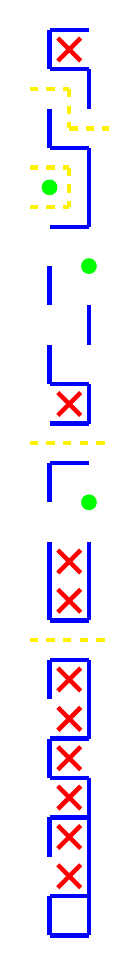
\begin{tikzpicture}[x=0.5cm, y=-0.5cm, ultra thick, blue]
% Walls
    \draw (0,0) -- (1,0);
    \draw (0,1) -- (1,1);
    \draw (0,3) -- (1,3);
    \draw (0,5) -- (1,5);
    \draw (0,9) -- (1,9);
    \draw (0,10) -- (1,10);
    \draw (0,11) -- (1,11);
    \draw (0,15) -- (1,15);
    \draw (0,16) -- (1,16);
    \draw (0,18) -- (1,18);
    \draw (0,19) -- (1,19);
    \draw (0,20) -- (1,20);
    \draw (0,22) -- (1,22);
    \draw (0,23) -- (1,23);
    \draw (0,0) -- (0,1);
    \draw (0,2) -- (0,3);
    \draw (0,6) -- (0,7);
    \draw (0,8) -- (0,9);
    \draw (0,11) -- (0,12);
    \draw (0,13) -- (0,15);
    \draw (0,16) -- (0,17);
    \draw (0,18) -- (0,19);
    \draw (0,20) -- (0,21);
    \draw (0,22) -- (0,23);
    \draw (1,1) -- (1,2);
    \draw (1,3) -- (1,5);
    \draw (1,7) -- (1,8);
    \draw (1,9) -- (1,10);
    \draw (1,13) -- (1,15);
    \draw (1,16) -- (1,18);
    \draw (1,19) -- (1,23);
% Pillars
    \fill[green] (0,4) circle(0.2);
    \fill[green] (1,6) circle(0.2);
    \fill[green] (1,12) circle(0.2);
% Inner points in accessible cul-de-sacs
    \node at (0.5,0.5) {};
    \node at (0.5,9.5) {};
    \node at (0.5,13.5) {};
    \node at (0.5,14.5) {};
    \node at (0.5,16.5) {};
    \node at (0.5,17.5) {};
    \node at (0.5,18.5) {};
    \node at (0.5,19.5) {};
    \node at (0.5,20.5) {};
    \node at (0.5,21.5) {};
% Entry-exit paths without intersections
    \draw[dashed, yellow] (-0.5,1.5) -- (0.5,1.5);
    \draw[dashed, yellow] (0.5,2.5) -- (1.5,2.5);
    \draw[dashed, yellow] (-0.5,3.5) -- (0.5,3.5);
    \draw[dashed, yellow] (-0.5,4.5) -- (0.5,4.5);
    \draw[dashed, yellow] (-0.5,10.5) -- (1.5,10.5);
    \draw[dashed, yellow] (-0.5,15.5) -- (1.5,15.5);
    \draw[dashed, yellow] (0.5,1.5) -- (0.5,2.5);
    \draw[dashed, yellow] (0.5,3.5) -- (0.5,4.5);
\end{tikzpicture}
\end{center}
\vspace*{\fill}

\end{document}
